\section{Sharing the Information}
As the network of ubiquitous computers grows bigger, the amount of context information will increase as well, and it becomes necessary to understand how this information can be shared. When billions of users and applications is connected to the infrastructure, it is important to get the most effective and scalable solution for storing and sharing this kind of data. Applications will need to be able to access data in real-time, so the users get the most updated context information. 

To share the information ubiquitous devices need a middleware, a platform that can run on the ubiquitous devices and enable information sharing. This middleware should be able to provide the functionality for collecting and sharing context information, it also needs to be able to share the context information in real-time. Because of the ubiquitous devices resource limitations it needs to be lightweight and use the resources in an efficient way. There are two approaches this middleware could use to share context information, centralized and distributed.

\subsection{Centralized}
With centralized middleware solutions, the data is hosted and managed on a server, and if a device needs to store or access context information it has to connect to this server. One advantage of the centralized approach is that a server can be updated, with new hardware and software, to improve its performance. 
However, a server can only handle a certain amount of requests per second. To handle the larger quantities of requests, more servers will be required causing the costs to increase with the amount of users. A centralized approach is vulnerable to failures like attacks and crashes. When the server goes down, users won't be able to retrieve context information. Some examples of Internet of Things middleware which use this approach are SenseWeb \cite{senseweb} and Xively \cite{xively}.

%\begin{figure}[t]
%	\centering
%    	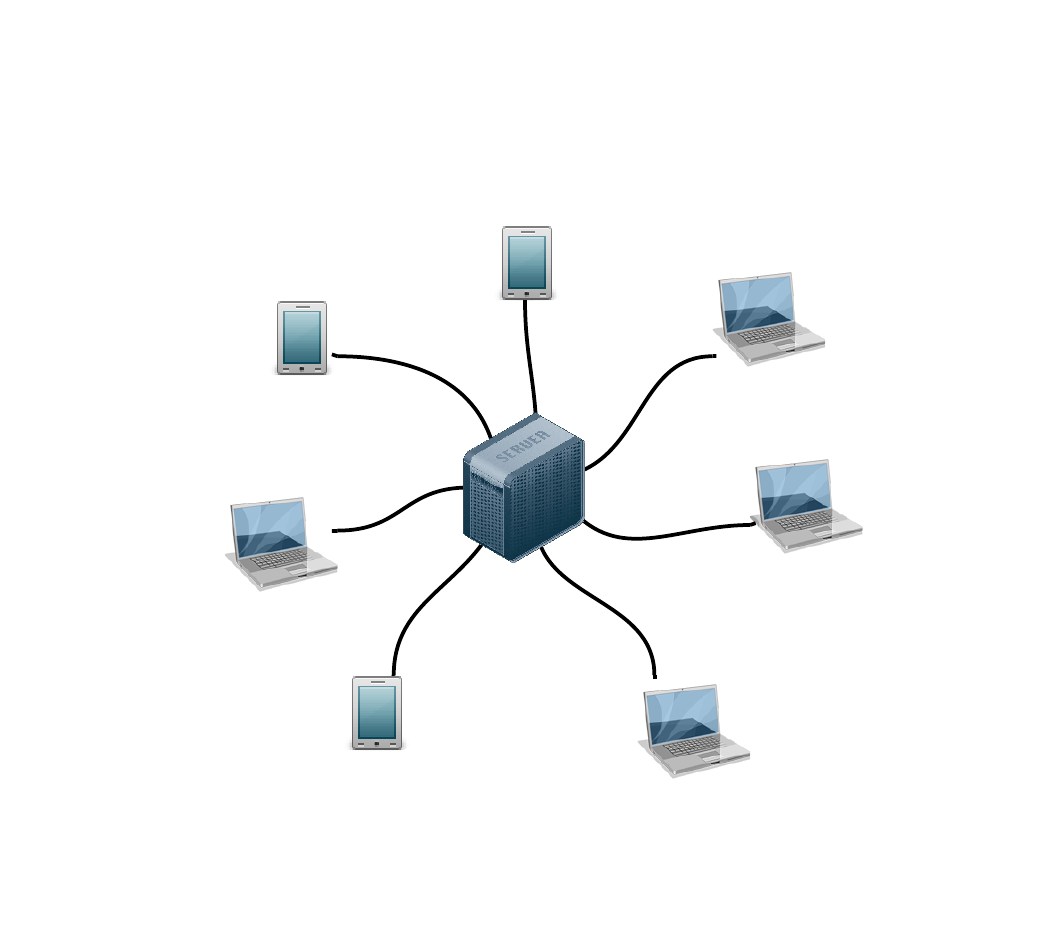
\includegraphics[scale=0.25]{part_2/sharing_the_information/Centralized.png}
%		\caption{Overview of a centralized network} 
%\end{figure}

\subsection{Distributed}
Distributed solutions allow computers / nodes to communicate with each other and share information and resources without using server computers. This is commonly used in file sharing software applications, such as Gnutella. Distributed solutions are more reliable and lack a single point of failure. Distributed solutions scale well compared to centralized solutions. Ubiware \cite{osterle2010memorandum} and MediaSense \cite{TheMediaSenseFramework} are both distributed Internet of Things middleware. 

%\begin{figure}[t]
%	\centering
%    	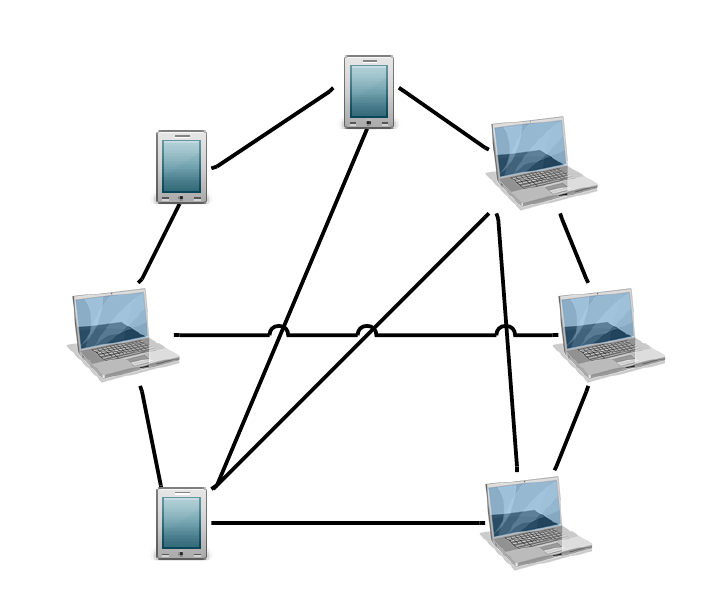
\includegraphics[scale=0.25]{part_2/sharing_the_information/Decentralized.png}
%		\caption{Overview of a decentralized network} 
%\end{figure}
